% \documentclass[12pt, twoside]{article}
\usepackage[letterpaper, margin=1in, headsep=0.2in]{geometry}
\setlength{\headheight}{0.6in}
%\usepackage[english]{babel}
\usepackage[utf8]{inputenc}
\usepackage{microtype}
\usepackage{amsmath}
\usepackage{amssymb}
%\usepackage{amsfonts}
\usepackage[nomessages]{fp} %\FPeval{\var-name}{2*sin(pi/6)}
\usepackage{siunitx} %units in math. eg 20\milli\meter
\usepackage{yhmath} % for arcs, overparenth command
\usepackage{tikz} %graphics
\usetikzlibrary{quotes, angles, arrows, arrows.meta}
\usepackage{graphicx} %consider setting \graphicspath{{images/}}
\usepackage{parskip} %no paragraph indent
\usepackage{enumitem}
\usepackage{multicol}
\usepackage{venndiagram}

\usepackage{fancyhdr}
\pagestyle{fancy}
\fancyhf{}
\renewcommand{\headrulewidth}{0pt} % disable the underline of the header
\raggedbottom
\hfuzz=2mm %suppresses overfull box warnings

\usepackage{hyperref}

\fancyhead[LE]{\thepage}
\fancyhead[RO]{\thepage \\ Name: \hspace{4cm} \,\\}
\fancyhead[LO]{BECA / Dr. Huson / Geometry\\*  Unit 1: Segments, length, and area\\* 11 Sept 2022}

\begin{document}

\subsubsection*{1.4 Classwork: Midpoints and bisectors}
\begin{enumerate}
\item Point $B$ is the midpoint of $\overline{AC}$, with $AB=x+5$, $BC=15$. First write an equation representing the situation, find $x$, then check it. \par \bigskip
    \begin{tikzpicture}
        \draw[fill] (0,0) circle [radius=0.05] node[below]{$A$};
        \draw[-, thick] (0,0)--(8,0);
        \draw[fill] (4,0) circle [radius=0.05] node[below]{$B$};
        \draw[fill] (8,0) circle [radius=0.05] node[below]{$C$};
        \node at (2,0.5) [above]{$x+5$};
        \node at (6,0.5) [above]{$15$};
        \draw (1.8,-0.2)--(1.9,0.2);
        \draw (2.1,-0.2)--(2.2,0.2);
        \draw (5.8,-0.2)--(5.9,0.2);
        \draw (6.1,-0.2)--(6.2,0.2);
    \end{tikzpicture} \vspace{2cm}

\item Given $M$ is the midpoint of $\overline{AB}$, $AM=5x+2$, $MB=22$.
    \begin{enumerate}
        \item Mark the diagram with the values and tick marks
        \item Write an equation and solve for $x$
        \item Check your result
    \end{enumerate} \bigskip
    \begin{center}
    \begin{tikzpicture}
        \draw [fill] (0,0) circle [radius=0.05] node[below]{$A$};
        \draw [-, thick] (0,0)--(7,0);
        \draw [fill] (3.5,0) circle [radius=0.05] node[below]{$M$};
        \draw [fill] (7,0) circle [radius=0.05] node[below]{$B$};
    \end{tikzpicture}
    \end{center} \vspace{2cm}

\item Point $E$ bisects $\overline{DEF}$ and $DE=2x-2$, $DF=20$. Find ${x}$. (show check)
\begin{flushleft}
\begin{tikzpicture}
    \draw[-, thick] (0,0)--(8,0);
    \draw[fill] (0,0) circle [radius=0.05] node[below]{$D$};
    \draw[fill] (4,0) circle [radius=0.05] node[below]{$E$};
    \draw[fill] (8,0) circle [radius=0.05] node[below]{$F$};
    \node at (2,0.3) [above]{$2x-2$};
    \draw[<->, dashed] (0,-1)--(8,-1);
    \node at (4,-1) [below]{$20$};
    \draw (1.8,-0.2)--(1.9,0.2);
    \draw (2.1,-0.2)--(2.2,0.2);
    \draw (5.8,-0.2)--(5.9,0.2);
    \draw (6.1,-0.2)--(6.2,0.2);
\end{tikzpicture}
\end{flushleft}
    
\newpage
\item Two line segments or angles of equal measure are $\rule{4cm}{0.15mm}$. \bigskip

\item Points on the same plane are $\rule{5cm}{0.15mm}$. \bigskip

\item Mark point $L$ on the ray exactly 8 centimeters from the endpoint $K$. (measure it) \par \bigskip
\begin{tikzpicture}
    \draw[thick, ->] (0,0)--(12,0);
    \draw[fill] (0,0) circle [radius=0.05] node[above]{$K$};
\end{tikzpicture} \bigskip

\item Name each object using symbolic notation. 
    \begin{enumerate}
    \begin{multicols}{3}
    \item \hspace{1cm}
        \begin{tikzpicture}
        \draw[<->, thick] (1,0)--(1,3);
        \draw[fill] (1,0.5) circle [radius=0.05] node[right]{$R$};
        \draw[fill] (1,2.5) circle [radius=0.05] node[right]{$S$};
        \end{tikzpicture}
    \item
      \begin{tikzpicture}
        \draw[-, thick] (1,0)--(0,2);
        \draw[fill] (1,0) circle [radius=0.05] node[below]{$P$};
        \draw[fill] (0,2) circle [radius=0.05] node[left]{$Q$};
      \end{tikzpicture}
    \item
      \begin{tikzpicture}
        \draw [->, thick] (0,0)--(-3,1.5);
        \draw [fill] (0,0) circle [radius=0.05] node[below]{$B$};
        \draw [fill] (-2,1) circle [radius=0.05] node[below]{$A$};
      \end{tikzpicture}
    \end{multicols}
    \end{enumerate} \vspace{1cm}

\item Two points $P(-12.2)$, $Q(-5.5)$ are shown on the number line. Find $PQ$. \par \smallskip
\begin{tikzpicture}[scale=0.5]
    \draw[<->] (-16.5,0)--(2.5,0);
    \foreach \x in {-16,-14,...,2}
        \draw[shift={(\x,0)}] (0pt,-3pt)--(0pt,3pt) node[below=5pt]{$\x$};
    \draw[fill] (-12.2,0) circle [radius=0.08] node[above]{$P(-12.2)$};
    \draw[fill] (-5.5,0) circle [radius=0.08] node[above]{$Q(-5.5)$};
\end{tikzpicture} \vspace{3cm}

\item Assume that Dr. Huson's rides to school straight north from 80th Street to 164th Street.
\begin{enumerate}[itemsep=1cm]
    \item How many blocks is his morning commute?
    \item On what street is Dr. Huson's half way each morning?
    \item In the afternoon return commute, what street is half way?
\end{enumerate}


\end{enumerate}
\end{document}